% !TeX program = xelatex
\documentclass[11pt,a4paper]{article}
\usepackage[margin=24mm]{geometry}
\usepackage{amsmath,amssymb,booktabs,longtable,array,graphicx,tikz}
\usetikzlibrary{arrows.meta,positioning}
\usepackage[hidelinks]{hyperref}
\usepackage{enumitem}
\setlist{itemsep=3pt,topsep=4pt}
\title{What Has Already Been Solved?\\A Focused Review of SCALE and Its Execution-Control Lineage}
\author{Internal research note}
\date{November 20, 2026}
\begin{document}
\maketitle
\noindent\textbf{Purpose.} Establish the boundaries of existing results before claiming
novelty for our sweep-based research. This note does not modify the manuscript,
implement a competing method, or independently reproduce published experiments.
Page numbers refer to PDF pages unless printed page numbers are supplied.

\section{Main findings}
\begin{enumerate}
\item Fixed paths, geometric interference, movement/waiting control, action
precedence, and safe asynchronous execution have an established literature.
Their combination alone is insufficient evidence of a new contribution.
\item MILP-based passage-order adjustment predates SCALE. SCALE explicitly
builds on SADG and claims extensions for heterogeneous motion conflicts,
conflict-checking efficiency, and a combined planning/execution architecture.
\item A cycle between whole robot paths is different from a cycle between
executable actions. Partial progress can eliminate the former without ever
executing the latter.
\item Start and final occupancy assumptions are central. Segment Graph explicitly
excludes interference with other robots' starts/goals in its non-conflicting
trajectory condition; it illustrates endpoint blocking without a graph cycle.
\item Published safety/liveness claims are conditional. They do not imply that
all geometric instances are solvable, every online planner is complete, or a
finite-horizon objective optimizes the entire operation.
\end{enumerate}

\section{The relevant research lineage}
The branches below represent explicit conceptual relationships, not a claim that
all methods share an identical mathematical model.
\begin{figure}[htbp]
\centering
\resizebox{\linewidth}{!}{%
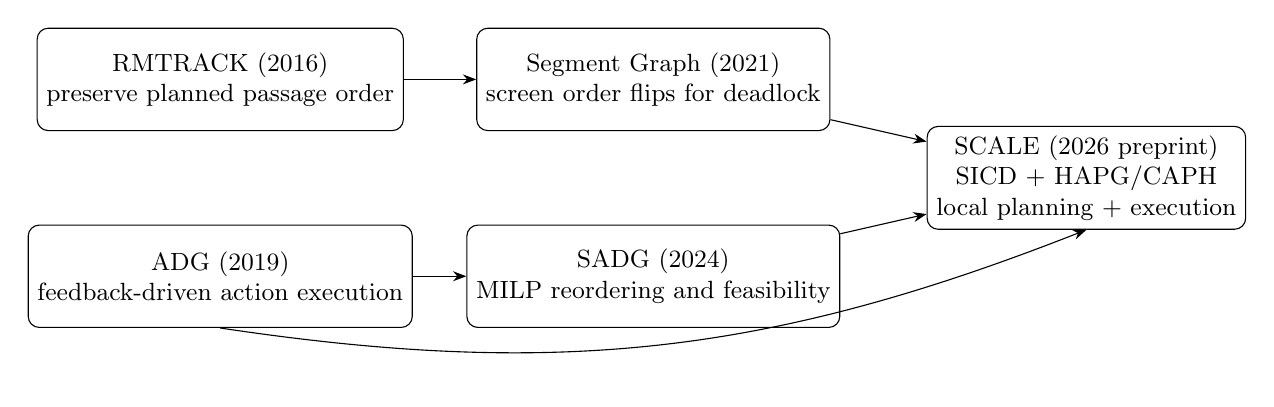
\begin{tikzpicture}[>=Stealth,box/.style={draw,rounded corners,align=center,minimum width=34mm,minimum height=13mm,font=\small}]
\node[box] (rm) at (0,0) {RMTRACK (2016)\\preserve planned passage order};
\node[box] (sg) at (5.5,0) {Segment Graph (2021)\\screen order flips for deadlock};
\node[box] (adg) at (0,-2.5) {ADG (2019)\\feedback-driven action execution};
\node[box] (sadg) at (5.5,-2.5) {SADG (2024)\\MILP reordering and feasibility};
\node[box] (scale) at (11,-1.25) {SCALE (2026 preprint)\\SICD + HAPG/CAPH\\local planning + execution};
\draw[->] (rm)--(sg);
\draw[->] (adg)--(sadg);
\draw[->] (sg)--(scale);
\draw[->] (sadg)--(scale);
\draw[->] (adg.south) to[bend right=15] (scale.south);
\end{tikzpicture}}
\caption{A focused map of the execution-control literature discussed here.}
\end{figure}

\section{What the predecessor papers establish}
\subsection{RMTRACK: preserve a known coordinated solution}
\textbf{Source:} \v{C}\'ap, Gregoire and Frazzoli~\cite{rmtrack}, Sections II--IV,
PDF pp.~2--5. The input is a jointly collision-free reference trajectory, not
arbitrary uncoordinated spatial paths. Robots are identical holonomic discs;
progress and stop/go decisions use discrete steps. Delays may stop advancement.

Theorem 1 establishes collision avoidance under the stated one-step margin
condition. Theorem 2 establishes eventual completion under non-prohibitive
disturbances. The key liveness argument enables at least a least-advanced
unfinished robot. This is not a proof that an arbitrary collection of paths can
be scheduled, nor resilience to a permanent disabling failure. The method keeps
the planned passage side/order around pairwise coordination obstacles.

\subsection{ADG: execute actions using completion reports}
\textbf{Source:} H\"onig et al.~\cite{adg}, Sections III--IV, PDF pp.~2--5.
The warehouse problem uses a four-connected grid and a well-formed infrastructure
assumption. ADG extracts own-action and inter-robot dependencies from a MAPF plan.
Runtime control uses completion reports rather than continual positions.
Consecutive forward commands can be combined while preserving individual
feedback. Planning can overlap execution through a dependency-aware commit cut.

The paper explicitly discusses a fully occupied $2\times2$ circular move:
a nominal synchronous MAPF solution need not admit robust asynchronous execution.
It detects such transitions through ADG cycles and restricts planning to avoid
them. Thus a feasible synchronous plan and a robust order-based execution are
not interchangeable notions.

\subsection{Segment Graph: when passage-order changes create deadlock}
\textbf{Source:} Coskun, O'Kane and Valtorta~\cite{sg}, Definitions 1--4 and
Theorems 1--4, PDF pp.~3--5. The model uses disc robots and discrete progress
along initially coordinated trajectories. Paths are partitioned at collision
segment boundaries, with own-path and obstacle-label precedence edges.

Definition 4 requires every path to avoid every other robot's initial and final
positions. Figure 4 shows why: a robot can finish and block another without a
graph cycle. Theorem 1 uses this endpoint assumption; cycle/deadlock statements
must be interpreted within the specified graph and control model. Theorem 4
gives a sufficient no-cycle condition when collision segments are disjoint.
Online repair rejects a proposed priority flip when it creates a cycle.

This is directly relevant to our earlier endpoint and separated-interference
discussions; it is not a universal solvability test for arbitrary path sets.

\subsection{SADG: optimize passage order without altering routes}
\textbf{Source:} Berndt et al.~\cite{sadg}, Sections III--VI, printed
pp.~1358--1367. Routes remain fixed. SE-ADG combines graph plans with spatial
exclusivity checks using an occupied area and Minkowski sums; calling it a
pure point-only representation would be inaccurate.

SADG constructs forward/reverse dependency alternatives, including shifted action
indices rather than an arbitrary arrow reversal. A MILP minimizes summed predicted
route completion times. Assumption 2 requires an initially acyclic SE-ADG.
Corollaries 4--5 relate feasible schedules to acyclicity; Propositions 1--2
establish recursive feasibility for shrinking/receding-horizon feedback.
Section VI includes dependency closure when extracting a finite horizon: local
acyclicity alone does not establish global acyclicity.

This is a conditional execution/reordering result, not initial path generation
or a universal guarantee for arbitrary cyclic dependency graphs.

\subsection{LaCAM*: the planning engine is a separate contribution}
\textbf{Source:} Okumura~\cite{lacam}, Sections 2--4 and Theorem 1,
printed pp.~244--247. LaCAM* searches joint graph configurations with lazy
successor generation and cost/parent updates. Its theorem proves completeness
and eventual optimality for the stated finite MAPF search model and accumulated
transition costs. Interrupting early yields an incumbent, not necessarily an
optimum; a timeout before a solution is not an infeasibility proof.

SCALE integrates its collision treatment with such existing planners.
LaCAM*'s original theorem cannot simply be transferred to an altered collision
model, horizon/group decomposition, and timeout fallback without checking the
new search coverage and assumptions.

\section{SCALE: a closer technical reading}
\subsection{Representation and planning}
The provided copy~\cite{scale} is the July 3, 2026 arXiv v2 manuscript; its
IEEE-style header has placeholder volume/issue fields. The supplied copy alone
does not establish journal acceptance.

Sections III--IV define a roadmap $G=(V,E)$ and continuous poses
$\gamma(\lambda)=(x(\lambda),y(\lambda),\theta(\lambda))$, with normalized
progress $\lambda$, not a fixed physical timestamp. Equation (1) sweeps a
robot-type footprint through translation and rotation, then adds a safety margin.
Different graph vertices or edges therefore need not mean disjoint physical
occupancy.

Section IV-A groups robots through detected cyclic dependencies over unreleased
bounded paths. Group regions are expanded on the roadmap, and local goals are
selected; obstructing idle robots may be assigned avoidance destinations.
Independent robots receive A* routes with contraflow/congestion costs.
The multi-robot part integrates SICD with graph-planning solvers.
This is an integrated route-repair and execution architecture, not fixed-route
execution alone.

\subsection{SICD: geometry reduced to finite occupancy sets}
Equation (3), p.~5, maps a sampled swept region to nearby roadmap vertices,
then represents their occupancy as bits. An incremental bitwise intersection
replaces repeated pairwise polygon queries during search. It is not a camera
image, nor necessarily a partition of the plane into regular cells.

The stated per-joint-transition bit-operation bound is
$O(N|V|/w_m)$, compared with the stated direct-polygon-check expression
$O(N^2 L c_{\rm poly})$. This comparison concerns conflict queries during
search; it does not bound all path planning, preprocessing, memory use, or
MILP optimization. Section IV-A.3 explicitly relies on complementary geometric
handling during execution. A proof that finite node/sweep sampling conservatively
captures every relevant continuous interaction is not supplied there in the form
of a sampling-density or geometric-coverage condition.

\subsection{HAPG, capsules, and switchable dependencies}
Algorithm 1, p.~3, accepts planned paths with precedence ranks and builds a
Hybrid Action-Precedence Graph. It is not the path planner. Own-action edges
preserve each path; inter-robot edges impose orders on conflicting actions.
Lemma III.2 assumes a feasible rank-consistent plan.

Section IV-B groups consecutive actions into capsules. A conflict signature
records which actions of one path conflict with an action of the other.
Constant-signature intervals and their conjugate spans generate candidate
capsule pairs. A switch is allowed only before the affected capsules start.
This is structurally close to reasoning about interfering subpaths, but is not
a search over all possible point-wait duplications.

\subsection{What the MILP does and does not optimize}
Equation (4), p.~7, chooses binary precedence orientations and continuous start/end
times for a bounded set of unreleased capsules:
\[
 \min \sum_{Q\in\mathcal Q_K^{\rm end}} T_g(Q).
\]
The constraints enforce durations, fixed orders, and one of two capsule passage
orders via big-$M$. The objective is summed predicted horizon-exit time, not
full-operation makespan. It is neither an exact full-Plant simulation evaluator
nor a joint optimization of all possible routes. Definition IV.2 estimates nominal
action duration from trajectory length and robot-type speed; Table II also lists
acceleration/braking limits for experimental robots. Consequently it is inaccurate
to describe the entire study as purely constant-speed, but the displayed MILP does
not contain explicit acceleration-state evolution or a trapezoidal profile model.

\subsection{The guarantee and the retry strategy}
Theorem IV.7, p.~7, argues collision/deadlock freedom for feasible planned paths
with valid capsule precedences. Accepted switches preserve temporal feasibility;
positive-duration cycles cannot satisfy the time inequalities. This is not a
proof that MILP can repair any arbitrary cyclic state.

Remark IV.1, p.~6, splits a failed local group, reduces the commitment horizon,
and relaxes the timeout before retrying. No finite retry bound or general
completeness theorem for this combined fallback is stated. A successful initial
plan, safety of a switch, eventual completion under disturbances, and guaranteed
success of the planning process are separate claims.

\subsection{What the experimental numbers mean}
Section V uses three robot types and simulated delay/loss/blockage settings.
The local planning evaluation includes 10,000 instances with 2--20 robots and
a 500 ms timeout. Its 90\% SICD/LaCAM* success rate is not a proof of universal
solvability. Execution-policy experiments use 50 solvable instances at each
group size 10--50. Section V-C reports a three-day, 300-robot system simulation;
Section V-D reports multi-day operation of 100 physical robots, about 30,000
tasks, and a 10 s scheduling period. These are different experiments, not a
300-robot physical deployment or a 10 ms event controller.

The copy does not identify a MILP solver/version, an optimality-gap policy,
a detailed authorization-time table, or all settings needed to reproduce the
full claimed deployment. The 700--1800 ms range refers to path planning;
authorization adds overhead. Report these as author-reported results, not our
independently reproduced measurements.

\section{Questions requiring clarification, not established refutations}
\begin{enumerate}
\item \textbf{Sampling and physical occupancy.} What geometric coverage or safety
margin prevents two overlapping swept regions from being missed by vertex
occupancy sampling? How is idle/final occupancy retained in every release check?
The text treats shortened horizon terminal vertices as persistent occupancy in
group formation, but the full implementation invariant is not specified.
\item \textbf{Capsule-pair closure.} Lemma IV.3's one-direction inclusion follows
from the stated signature span. Its claimed symmetric inclusion requires mutual
closure. The prose mentions a mutual construction but does not spell out an
iterated closure or a separate reverse-signature validation algorithm.
\item \textbf{Safe horizon boundaries.} Which global dependency conditions prevent
bounded-horizon switching from introducing a cycle through excluded actions?
Compare this specifically with SADG's Section VI closure construction.
\item \textbf{Switchability and progress.} Lemma IV.4 excludes two singleton
capsules from switching; the necessity of this restriction needs explanation.
Acyclicity rules out circular waiting, but finite completion also requires finite
action execution and eventual delivery/processing of enabling feedback.
\item \textbf{Optimization reproducibility.} Which solver, time anchors, incumbent
fallback, big-$M$ bounds, tolerance, timeout, and stopping criteria were used?
Equation (4) alone is a compact formulation, not a complete executable specification.
\end{enumerate}
A missing explanation is not itself a counterexample. None of these questions
has been experimentally established here as a failure of the authors' method.

\section{Implications for our work}
\subsection{Three different cycles}
\begin{enumerate}
\item \textbf{Undirected sweep overlap:} indicates interaction, not precedence.
\item \textbf{Whole-path serial requirements:} asks whether a robot can finish its
entire route before another. A cycle can disappear when routes are split.
Our two-robot $A\to C$, $B\to F$, $C\to E$ example belongs here.
\item \textbf{Action-level finish-before-start requirements:} an active directed
cycle with positive durations is temporally infeasible under that policy.
Changing the order, segmentation, or routes changes the problem; it does not
execute the unchanged cyclic dependency graph.
\end{enumerate}
These graph types must never be substituted for one another in a theorem.

\subsection{What our current results actually say}
Our endpoint test $F_{ij}$ is a sufficient two-order serial test for general
paths, not a general feasibility oracle. The acyclic whole-path requirement
construction is sufficient. Our finite constituent search can return a validated
partial-progress tuple outside that construction; completeness is confined to
its permitted constituents, point waits, and conservative all-pair stage-sweep
tests. It does not establish completeness over arbitrary continuous stopping
locations, synchronized moving-body schedules, or all physical executions.

Point-wait duplication resembles waiting in existing coordination-space
schedules. Sweep merging must be compared with already-established queued-action
combination and spatial action grouping. DEVS and interactive animation are useful
implementation features, not automatic theoretical novelty. Our representation
can still be valuable as a derivation and engineering artifact even if its
underlying principle is already known.

\subsection{An unresolved implementation audit}
Our current finite search enumerates selected robot subsets, including simultaneous
constituent choices. Earlier conversational descriptions sometimes reduced it to
one mover and one waiter. These are not identical algorithm definitions.
For a stage whose full component sweeps are pairwise disjoint, sequentializing
those components is safe because all waiting footprints are subsets of the
stage sweeps. Thus a selected-subset stage can be serialized at the geometric
level, assuming the constituent endpoints admit stopping. Implementation-level
point/edge token consumption and movement feasibility must still be checked.
Do not claim broader continuous-motion serializability from this limited fact.

\subsection{Useful next comparisons}
\begin{enumerate}
\item Put our endpoint assumptions beside Segment Graph Definition 4 and its
Figure 4 endpoint-blocking counterexample. Determine whether we have a genuine
extension or simply different sufficient conditions.
\item Map one of our alternating-progress witnesses to an action/segment graph.
Identify exactly which vertices and edges it would generate in each method.
\item Compare certificate retention with SADG recursive feasibility: both retain
a compatible completion route, but their state spaces and allowed switches differ.
\item Test identical fixed paths, footprints, admissible stopping positions and
motion models before making performance claims. Separate construction cost,
execution computation, sampled validation, and rendering.
\item Only then select a new theorem or PathPlanner objective. A different
objective or a new terminology for old operations is not sufficient evidence.
\end{enumerate}

\section{Reading record and limits}
This review inspected the local SCALE manuscript and the formal models,
algorithms, key proof sections and experiment descriptions of the five sources
below. It is not a proof-by-proof equivalence theorem or an independent execution
of their software. Public PDFs were retrieved from the listed author,
institution/project or proceedings sources. An author-hosted Segment Graph copy
has an anonymous review header; bibliographic attribution is corroborated by
SCALE's reference [29]. SADG's final volume year is 2024 although its DOI and
online publication are dated 2023. The working RMFS paper and simulation code
were not changed during this review.

\begin{thebibliography}{9}
\bibitem{scale} B. Cao, ``From Real-Time Planning to Reliable Execution: Scalable
Coordination for Heterogeneous Multi-Robot Fleets in Industrial Environments,''
arXiv:2607.00591v2, July 3, 2026. Provided local copy:
\path{Real-TimePlanningTo_IEEE_TII.pdf}. \url{https://arxiv.org/abs/2607.00591v2}.
\bibitem{rmtrack} M. \v{C}\'ap, J. Gregoire, and E. Frazzoli, ``Provably Safe and
Deadlock-Free Execution of Multi-Robot Plans under Delaying Disturbances,''
arXiv:1603.08582, 2016. \url{https://arxiv.org/abs/1603.08582}.
\bibitem{adg} W. H\"onig, S. Kiesel, A. Tinka, J. W. Durham, and N. Ayanian,
``Persistent and Robust Execution of MAPF Schedules in Warehouses,''
\emph{IEEE Robotics and Automation Letters}, 4(2), 1125--1131, 2019.
\url{https://whoenig.github.io/publications/2019_RA-L_Hoenig.pdf}.
\bibitem{sg} A. Coskun, J. M. O'Kane, and M. Valtorta, ``Deadlock-Free Online Plan
Repair in Multi-robot Coordination with Disturbances,'' FLAIRS, 2021.
\url{https://jokane.net/pubs/CosOKaVal21.pdf}.
\bibitem{sadg} A. Berndt, N. van Duijkeren, L. Palmieri, A. Kleiner, and T. Keviczky,
``Receding Horizon Re-Ordering of Multi-Agent Execution Schedules,''
\emph{IEEE Transactions on Robotics}, 40, 1356--1372, 2024.
\url{https://doi.org/10.1109/TRO.2023.3344051}.
\url{https://darko-project.eu/wp-content/uploads/papers/2024/Receding_Horizon_Re-Ordering_of_Multi-Agent_Execution_Schedules.pdf}.
\bibitem{lacam} K. Okumura, ``Improving LaCAM for Scalable Eventually Optimal
Multi-Agent Pathfinding,'' IJCAI, 243--251, 2023.
\url{https://www.ijcai.org/proceedings/2023/0028.pdf}.
\end{thebibliography}
\end{document}
